% TEXINPUTS=.:$HOME/git/bvtex: latexmk  -pdf <main>.tex
\documentclass[xcolor=dvipsnames]{beamer}

\input{defaults}
\input{beamer/preamble}

\setbeamertemplate{navigation symbols}{}
% \setbeamertemplate{background}[grid][step=1cm]

\usepackage{siunitx}
\usepackage{xmpmulti}
\usepackage[export]{adjustbox}
\usepackage{ulem}
\usepackage[outline]{contour}
\usepackage{tikz}
\usetikzlibrary{shapes.geometric, arrows}
\usetikzlibrary{positioning}

\definecolor{bvtitlecolor}{rgb}{0.98, 0.92, 0.84}
\definecolor{bvoutline}{rgb}{0.1, 0.1, 0.1}

\renewcommand{\bvtitleauthor}{Brett Viren}
\renewcommand{\bvtit}{LARF}
\renewcommand{\bvtitle}{\LARGE 3D Detector Response Calculations\\Using \textbf{B}oundary \textbf{E}lement \textbf{M}ethod}
\renewcommand{\bvevent}{BNL-$\mu$Boone\\10 Aug 2016}
\renewcommand{\bvbeamerbackground}{}

\newcommand{\microboone}{MicroBooNE\xspace}


\begin{document}
\input{beamer/title.tex}


\begin{frame}
  \frametitle{Overview}
  \begin{itemize}
  \item Status report with focus on active, technical problems.
  \end{itemize}
\end{frame}


\begin{frame}
  \frametitle{MicroBooNE Geometry Patch}

  \begin{columns}
    \begin{column}{0.5\textwidth}
      \begin{center}
        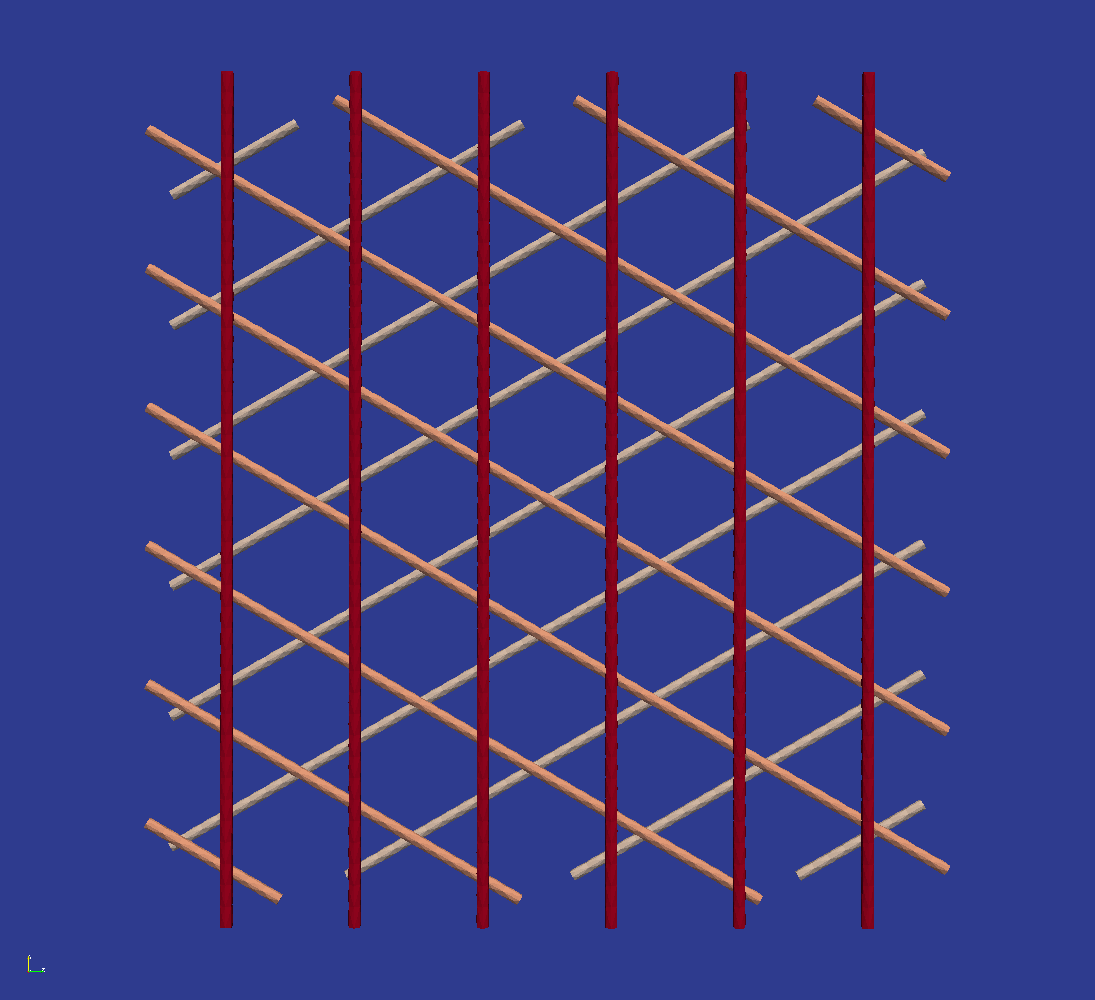
\includegraphics[width=\textwidth]{wires-flat.png}
      \end{center}
    \end{column}
    \begin{column}{0.5\textwidth}
      \begin{center}
        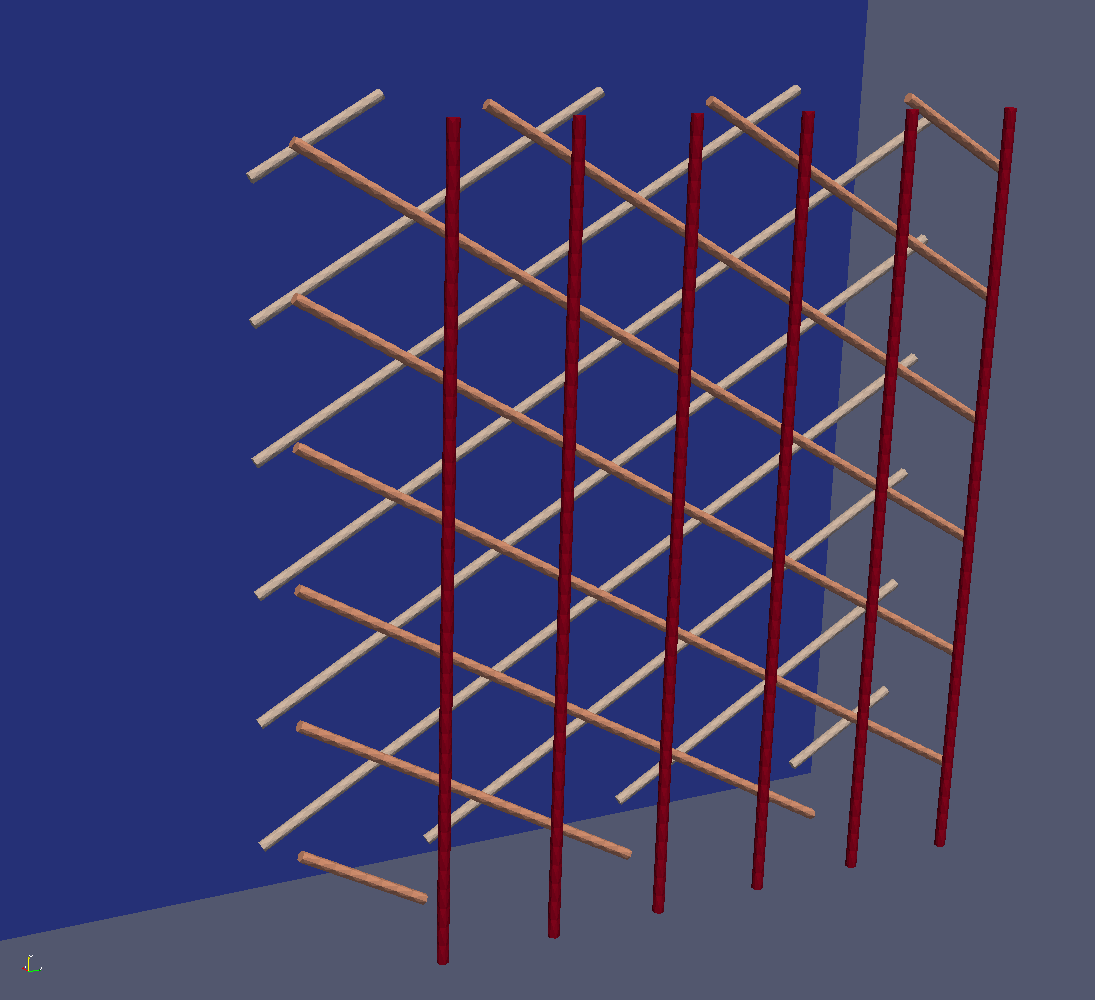
\includegraphics[width=\textwidth]{wires-iso.png}
      \end{center}
    \end{column}
  \end{columns}
  

  \begin{itemize}
  \item Wires parameterized by pitch, angle, bounding box, radius.
  \item Single $40 \times 40$mm plane at +20mm for drift potential
  \item Wire planes fill a $20 \times 20 \times 6$ mm box
  \end{itemize}


\end{frame}

\begin{frame}
  \frametitle{V-plane $\vec{E}_{weight}$ Slices}
  \begin{center}
    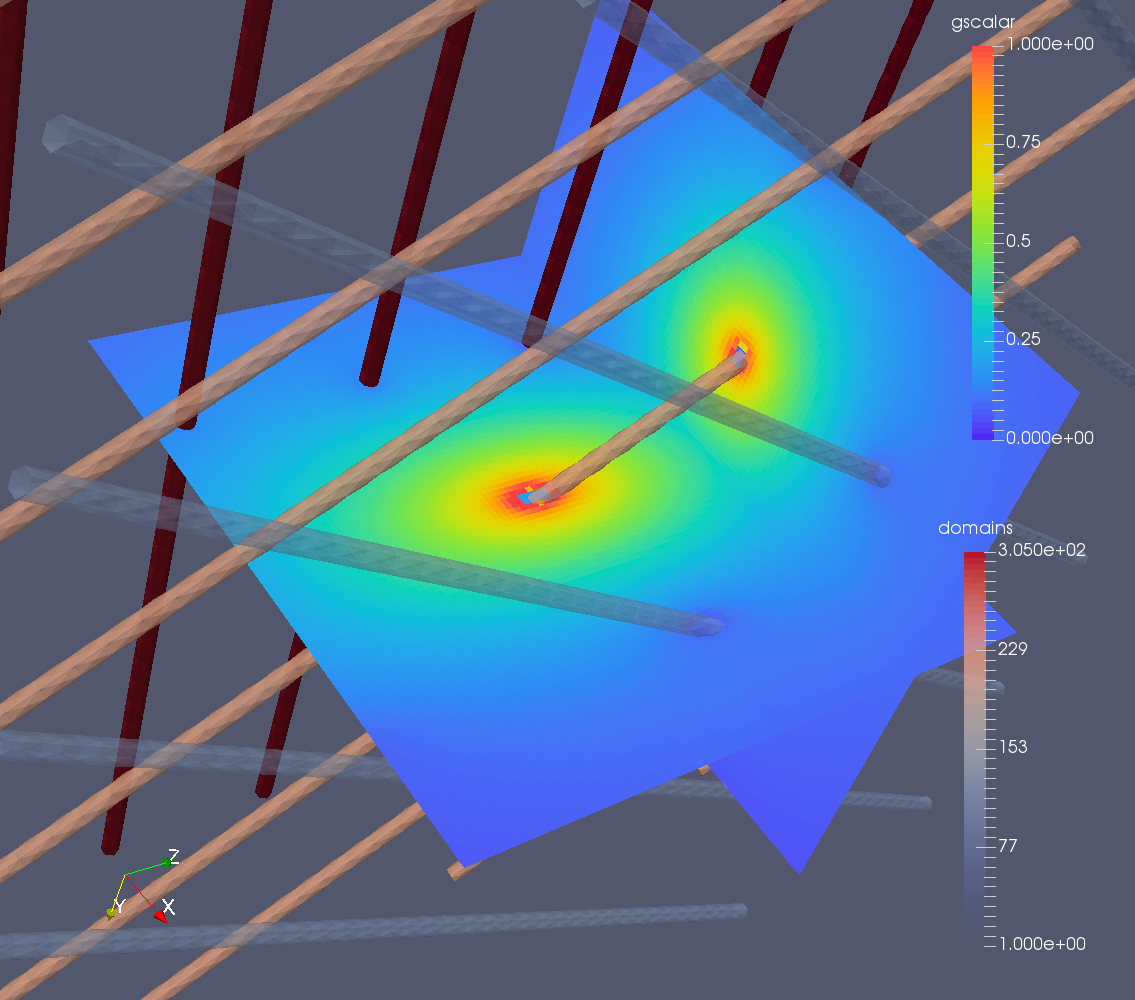
\includegraphics[width=0.6\textwidth]{cap-vweight-field-fine-slices.png}
  \end{center}

  \begin{itemize}\footnotesize
  \item Slices in X-Z and X-Y planes.
  \item \textbf{Note:} mismatchs between evaluated voxel grid and wire mesh.
  \end{itemize}
\end{frame}

\begin{frame}
  \frametitle{Paraview stepping from line source}
  \begin{center}
    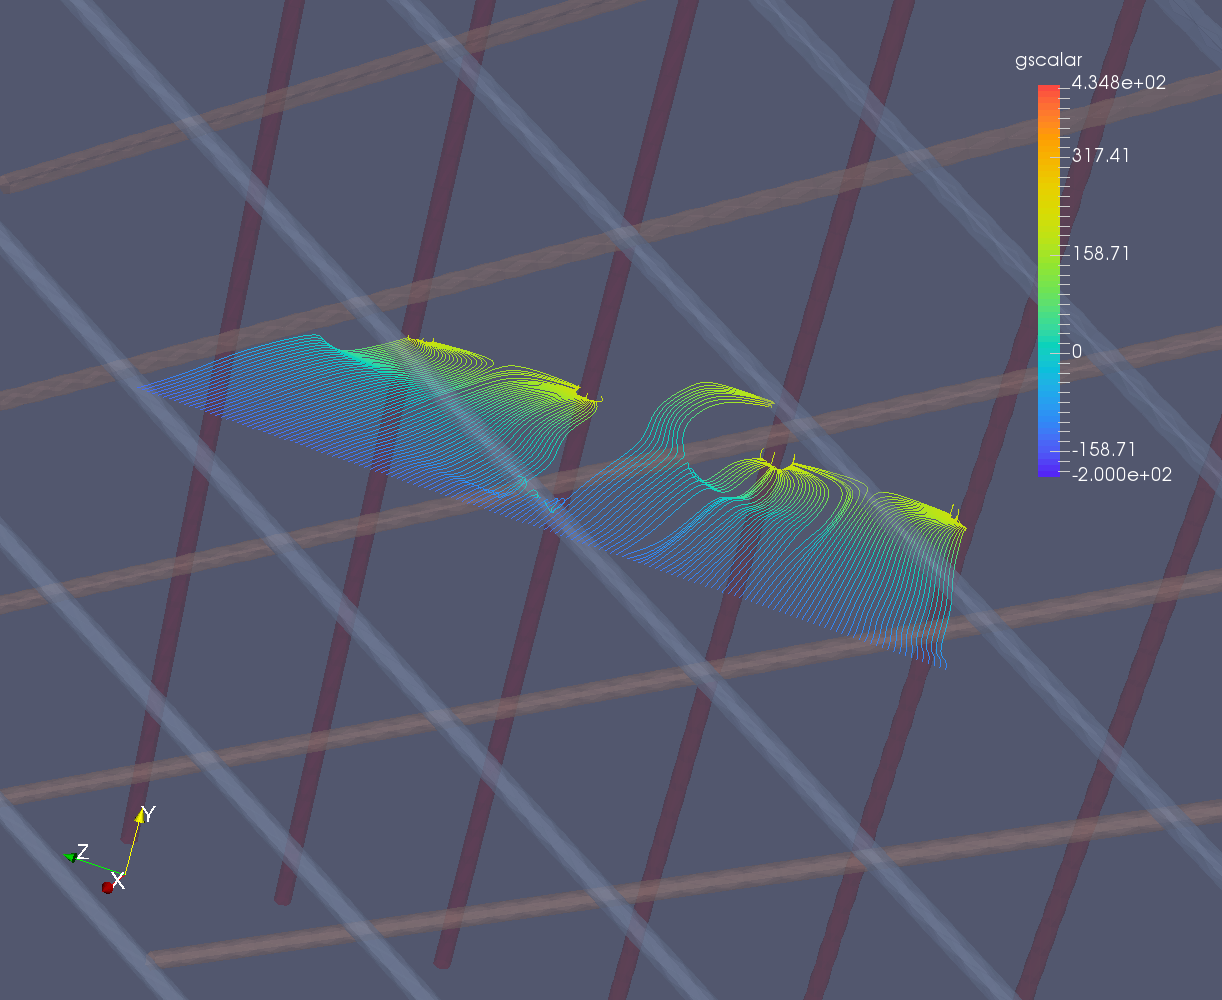
\includegraphics[width=0.55\textwidth]{track-drift-2.png}
  \end{center}

  \begin{itemize}\footnotesize
  \item Line source 2mm in front of U-plane,  paths colored by drift potential.
  \item U-plane transparency violated due to imprecision right near U-wire.
  \item Likely, \textbf{voxelization} is mostly to blame.  \textbf{Finite mesh size}
    and \textbf{gradient not respecting wire boundary} are 2nd order culprits.
  \end{itemize}
\end{frame}

\begin{frame}
  \frametitle{Mesh Sampling Precision Reminder} 
  \begin{columns}
    \begin{column}{0.3\textwidth}
      \begin{center}
        A particularly egregious example. 
      \end{center}
    \end{column}
    \begin{column}{0.7\textwidth}
      \begin{center}
        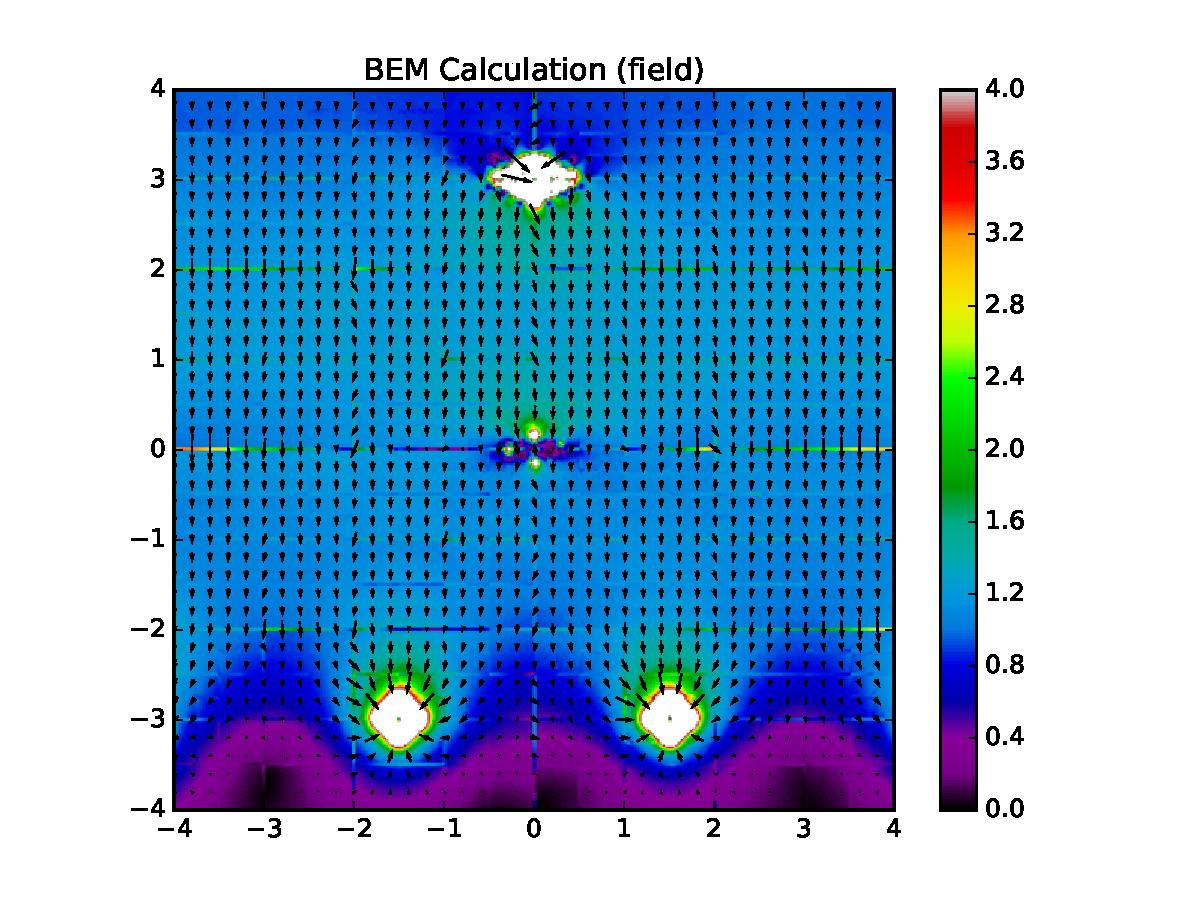
\includegraphics[height=5cm,clip,trim=2cm 1cm 2cm 1cm]{uboone-drift-field-tight.pdf}    
      \end{center}
    \end{column}
  \end{columns}
  \begin{itemize}\footnotesize
  \item BEM++ allows setting ``Gaussian Quadrature Order''.
  \item 3 knobs: number of samples of boundary conditions on each mesh triangle
    for ``near'', ``middle'' and ``far'' ranges.
  \item Large scale discontinuity artificats due to shifting between these ranges.
  \end{itemize}
\end{frame}

\begin{frame}
  \frametitle{Initial Response Functions (given known issues)}
  
  \footnotesize

  \begin{center}
    Preliminary and Subject to Change!

    \includegraphics[width=0.3\textwidth]{prec-wresponse-hit.pdf}%
    \includegraphics[width=0.3\textwidth]{prec-uresponse-hit.pdf}%
    \includegraphics[width=0.3\textwidth]{prec-vresponse-hit.pdf}

    Collection and U and V Induction.  Central and nearest neighbor wires.

    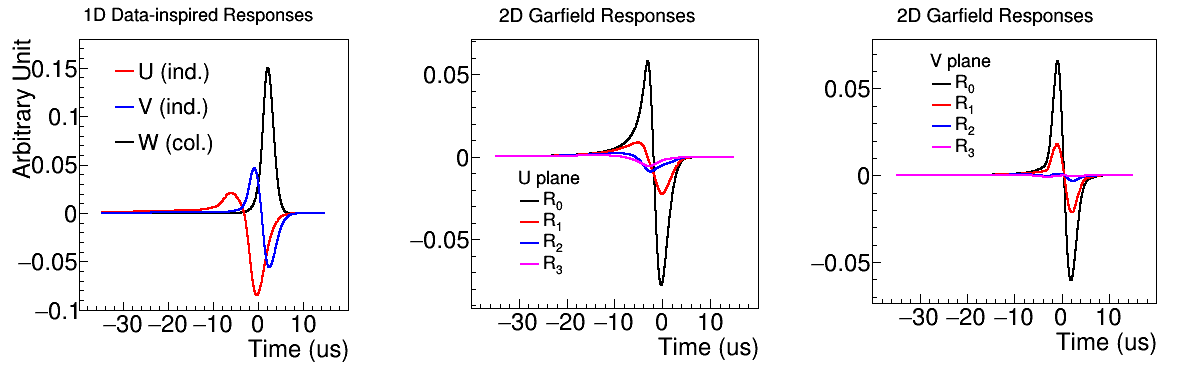
\includegraphics[width=0.7\textwidth]{overall_response.png}

    Data inspired and 2D Garfield calculations.
  \end{center}

\end{frame}

\begin{frame}
  \frametitle{Stepping with on-demand field eval}
  \includegraphics[width=\textwidth,clip,trim=2cm 8cm 2cm 8cm]{rogue-steps-low-quadrature.png}
  \begin{itemize}\footnotesize
  \item $\sim$20cm paths, color is drift potential, 1mm grid starting points
  \item Uses \textbf{on-demand field evaluations}
  \item Still \textbf{point-and-shoot} stepping (every 0.1us).
  \item Still \textbf{low Gaussian Quadrature precision}.
  \item Still \textbf{ignores wire hits}.
  \end{itemize}
\end{frame}


\begin{frame}
  \frametitle{To Do - fix/tune/optimize/test}
  \begin{itemize}
  \item \sout{Change from voxelized $\phi_{drift}$ to \textbf{on-demand}.}(done)
    \begin{itemize}\footnotesize
    \item Requires much less RAM and CPU for given spatial resolution.
    \item But, does evaluation + stepping together (no eval result
      caching)
    \item Each point uses 7 drift-potential evaluations to get gradient for $\vec{E}_{drift}$.
    \end{itemize}
  \item \sout{Replace point-and-shoot with \textbf{Runge-Kutta 5th order}}(ready)
    \begin{itemize}\footnotesize
    \item $\sim 6\times$ more CPU needed, tradeoffs to consider:
      \begin{itemize}\scriptsize
      \item Force step size to desired (eg, 0.1$\mu$s steps in time): Slow!
      \item Use adaptive error control, bigger steps in general but
        then, spline fit and sample: Fast but is it accurate,
        especially at the wires?
      \end{itemize}
    \end{itemize}
  \item \sout{Increase \textbf{Gaussian-quadrature order}.}(cfg parameter)
    \begin{itemize}\footnotesize
    \item Requires a ``few'' $\times$ more CPU (I've not carefully measured)
    \item Hopefully fixes the abrupt shifts in field.
    \end{itemize}
  \item Geometry.  Need to:
    \begin{itemize}\footnotesize
    \item be able to query geometry at step time to stop ``hit'' paths.
    \item enlarge geometry to +/- 10 wires (Yichen+Xin's work).
    \item enlarge ``cathode'' even more to provide more parallel drift field.
    \end{itemize}
  \end{itemize}
\end{frame}


\begin{frame}
  \frametitle{Leon's Advances with FEM}
  \begin{center}
    \href{http://microboone-docdb.fnal.gov:8080/cgi-bin/ShowDocument?docid=6236}{DocDB 6236}    
  \end{center}

  2D comparison with garfield
  \begin{itemize}
  \item Good looking current waveforms
  \item Found a time offset difference.
  \item Wants Garfield's steps $(\vec{r},t)$ for detailed comparison\\
    (Yichen, help?)
  \end{itemize}
  3D uBoone
  \begin{itemize}
  \item Can do drifts over ``unit cell'' ($\sim 3\times 6$ mm)
  \item Drift paths look good and ``less weird'' than my current ones.
    \begin{itemize}\footnotesize
    \item Ie, straight and parallel in region away from wires
    \end{itemize}
  \end{itemize}
\end{frame}



\begin{frame}
  \begin{center}
    FIN
  \end{center}
\end{frame}




\begin{frame}[fragile]
  \frametitle{Boundary Element Method (BEM) Overview}
  \begin{enumerate}  \footnotesize
  \item Discretize (mesh) boundary electrode \textbf{surfaces}.
  \item Define (Dirichlet) scalar potential on each mesh element (triangle).
  \item Fit (Neumann) surface-normal boundary field.
  \item Integrate Laplace equation $\nabla^2\phi=0$, evaluate at boundary.
  \item Evaluate solution at points in the volume.
  \end{enumerate}

  \vfill

  \footnotesize

  Compare BEM and FEM:

  \begin{center}

    \begin{tabular}[h]{rcc}
      & BEM & FEM \\
      \hline
      domain: & 2D surface mesh & 3D volume mesh \\
      easy: & away from surface & near to surface \\
      fits: & boundary-normal field & volumetric field \\
      eval: & arb. volume point & volume mesh points \\
      \hline
      both: & \multicolumn{2}{c}{CPU and memory intensive, limited geometries} \\
      external: & \multicolumn{2}{c}{stepping and averaging current responses} \\
    \end{tabular}
  \end{center}

\end{frame}

\begin{frame}
  \frametitle{General Calculation Overview}
  High-level steps:
  \begin{itemize}
  \item Drift fields: $\phi_{drift} \to \vec{E}_{drift} \to \mu \to \vec{v}_{drift} \to$ \textbf{paths}: $\{p\}$
    \begin{itemize}\footnotesize
    \item $\vec{v}_{drift} = \mu(E_{drift}) \vec{E}_{drift}(\vec{r}(t))$
    \item Get path $\vec{r}_p(t)$ by stepping through velocity field $\vec{v}_{drift}$.
    \end{itemize}

  \item Shockley-Ramo ``\textbf{weighting}'' potential for electrode $k$
    \begin{itemize}\footnotesize
    \item $\phi_{weight,k} \to \vec{E}_{weight,k}$
    \item Electrode $k$ at 1V, all others at 0V.
    \end{itemize}
  \item \textbf{Current on wire} $k$ due to charge moving along path $p$: 
    \begin{itemize}\footnotesize
    \item $i_{k,p}(t) = q \vec{E}_{weight,k} \cdot \vec{v}_{drift}|_p$
    \end{itemize}
  \item \textbf{Response function} for wire $k$ is average over paths: 
    \begin{itemize}\footnotesize
    \item $<i_{k}(t)> = \frac{1}{N}\sum_{p=1}^N i_{k,p}(t)$
    \end{itemize}
  \end{itemize}
  \vfill
  \footnotesize
  $\rightarrow$ for now: paths start on 1mm grid, 16mm in front of
  U-plane, 

  $\rightarrow$ response is average over paths in half-pitch ``wire region''
\end{frame}

\begin{frame}
  \frametitle{Wire Meshes}

  \footnotesize

  \begin{columns}
    \begin{column}{0.3\textwidth}
      \begin{center}
        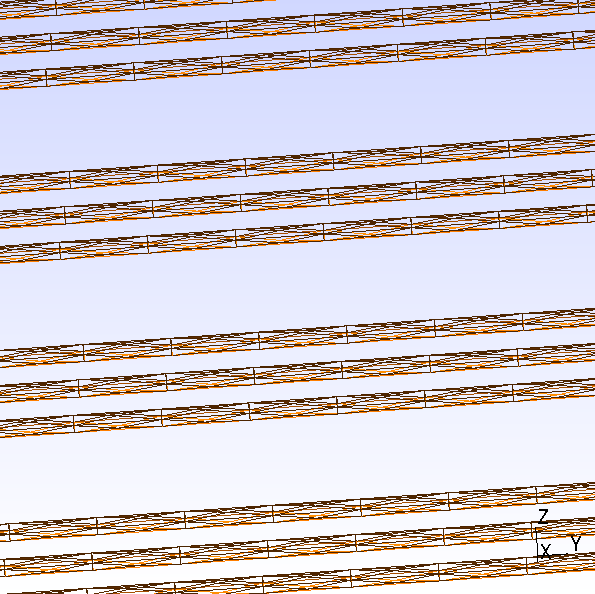
\includegraphics[height=0.4\textheight]{parallel-mesh.png}      
        
        ``Parallel'':\\3mm pitch and gap\\all wires parallel
      \end{center}
    \end{column}
    \begin{column}{0.3\textwidth}
      \begin{center}
        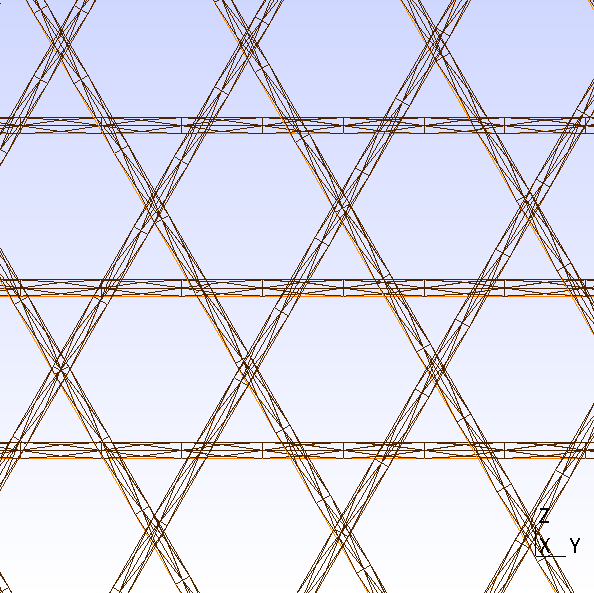
\includegraphics[height=0.4\textheight]{uboone-mesh.png}      

        ``MicroBooNE'':\\3mm pitch and gap\\$60^\circ$ angles for U/V.
      \end{center}
    \end{column}
    \begin{column}{0.3\textwidth}
      \begin{center}
        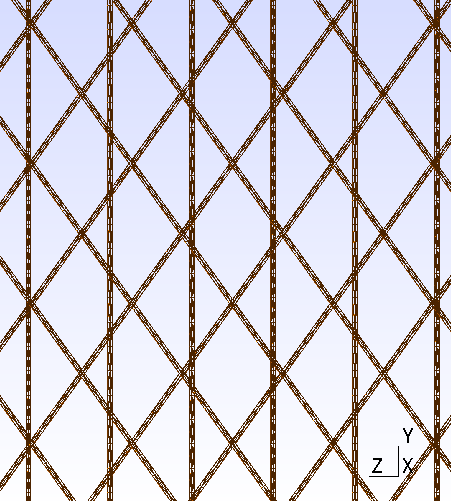
\includegraphics[height=0.4\textheight]{dune-mesh.png}      

        ``DUNE'':\\5mm pitch and gap\\$35.7^\circ$ angles for U/V.
      \end{center}
    \end{column}
  \end{columns}

  \vspace{4mm}

  \begin{itemize}
  \item ``Parallel'' used to reproduce 2D calculations. 
  \item Geometry parameterized to facilitate exploring different configurations.
  \end{itemize}

\end{frame}


\begin{frame}
  \frametitle{Parallel Wires - Slice Through Weighting Potentials}
  \begin{columns}
    \begin{column}{0.5\textwidth}
      \begin{center}
        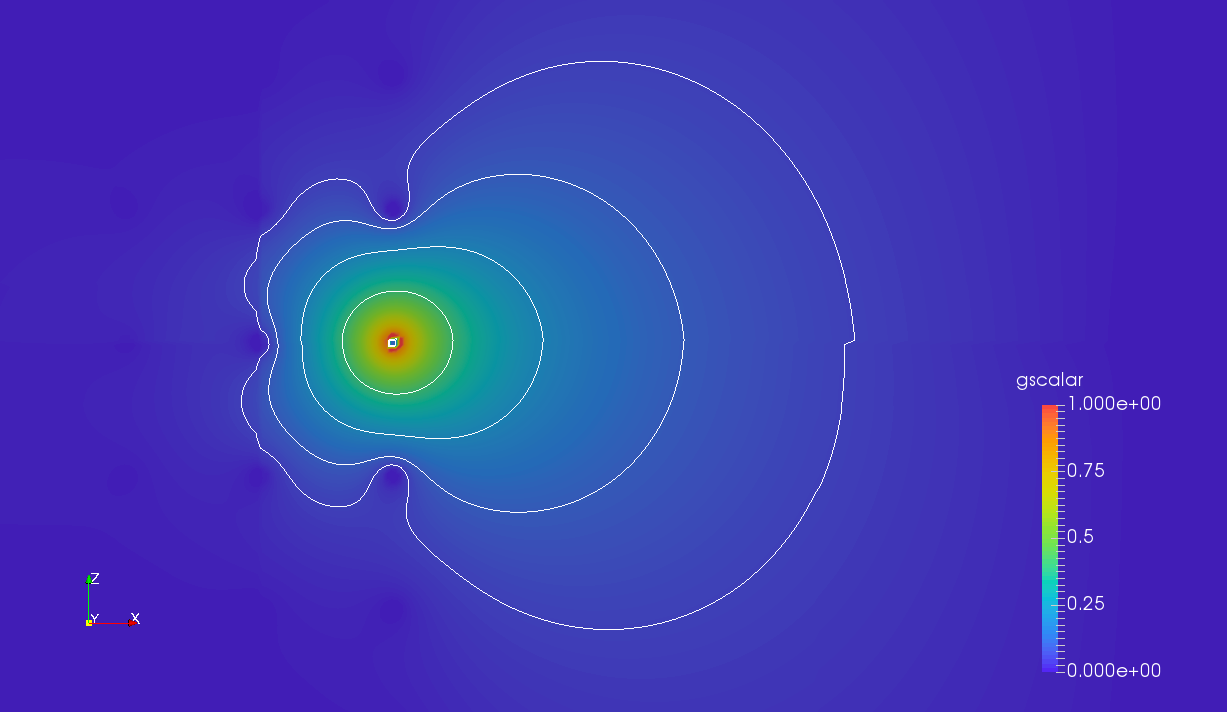
\includegraphics[height=3.5cm]{twodee-fine-u7.png}        
      \end{center}
    \end{column}
    \begin{column}{0.5\textwidth}
      \begin{center}
        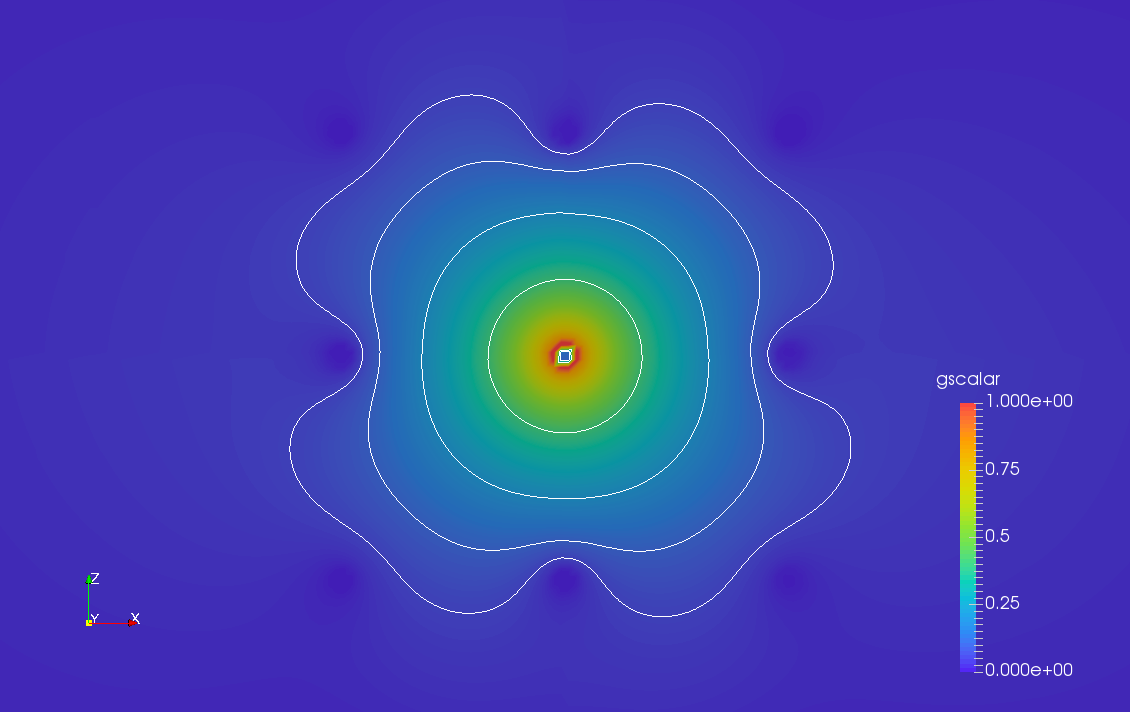
\includegraphics[height=3.4cm]{twodee-fine-v7.png}        
      \end{center}
    \end{column}
  \end{columns}
  \vspace{-1cm}
  \begin{columns}
    \begin{column}{0.5\textwidth}
      \begin{center}
        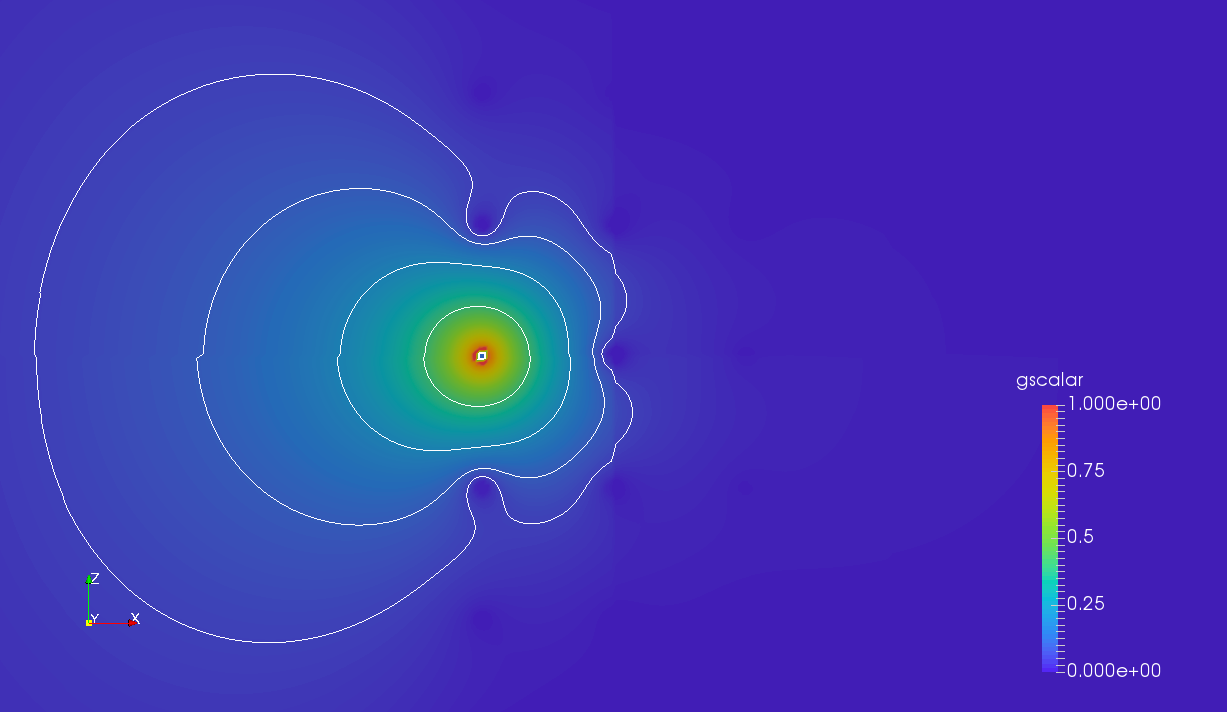
\includegraphics[height=3.5cm]{twodee-fine-w7.png}        
      \end{center}
    \end{column}
    \begin{column}{0.5\textwidth}
      \begin{itemize}\scriptsize
      \item U and W (left) and V (above) planes.
      \item X-Z slices through plane of symmetry.
      \item Lines: 5\%, 10\%, 20\%, 40\% weights.
      \item Initial qualitative agreement with Garfield 2D calculations.
      \item[$\rightarrow$] more exhaustive comparisons needed,
        but satisfactory enough to push on.
      \end{itemize}
    \end{column}
  \end{columns}

\end{frame}


\begin{frame}
  \frametitle{The Software}
  \begin{center}
    \url{https://github.com/brettviren/larf}
  \end{center}

  \begin{itemize}
  \item Expect a name change!
  \item Ready for other users and developers, \textbf{welcome!}
  \item Interfaces: \textbf{simple command line program} or 
    \textbf{Python modules}.
  \item Supports fantastic \textbf{Paraview} visualization app.
  \item Provides various ``management systems'': configuration, data
    storage, result provenance, workflow.
  \end{itemize}

  $\rightarrow$ Warning: \textbf{documentation is trailing code
    development} so let me know if you are interested in
  using/developing and I'll do some freshening.

\end{frame}


\end{document}
%%% Local Variables:
%%% mode: latex
%%% TeX-master: t
%%% End:
